
\section{The big picture}
Basic though it may seem, the combined model of algebra is to sequence the 
invention of new numbers, learn to compute with them, find relatinships 
between solutions, and use that to reinvent numbers.
\begin{center}
    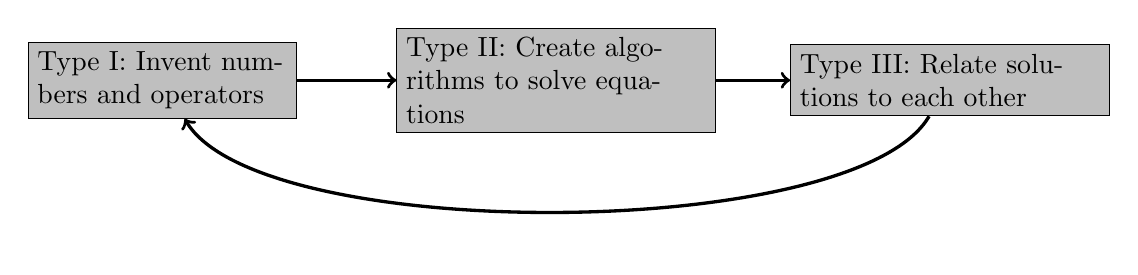
\begin{tikzpicture}
        \node[text width=1.25in, draw,fill=black!25] (a) at (0,0) {Type I: Invent numbers and operators};
        \node[text width=1.5in, draw,fill=black!25] (b) at (5,0) {Type II: Create algorithms to solve equations};
        \node[text width=1.5in, draw,fill=black!25] (c) at (10,0) {Type III: Relate solutions to each other};
        % \draw[very thick,->] (-4,0) -- (a);
        \draw[very thick,->] (a) -- (b);
        \draw[very thick,->] (b) -- (c);
        \draw[very thick,->] (c) edge[looseness=0.5,out=-120,in=-60] (a);
    \end{tikzpicture}
\end{center}


Yet to get started we better understand what it means to substitute 
for variables that can be $+$ signs and $=$ signs.

% \subsection{Questions}
% \begin{enumerate}
%     \item What is an equation?
%     \item What is a formula?
%     \item What is a variable?
%     \item Is substitution just replacing one symbol by another?
%     \item Why is $f(x)=x+c$ obviously a function when $f(a/b)=a+b$ is not?
%     \item 
% \end{enumerate}